%%%%%%%%%%%%%%%%%%%%%%%%%%%%%%%%%%%%%%%%%%%%%%
%                insertmeeting
% 1) Title (something creative & funny?)
% 2) Date (MM/DD/YYYY)
% 3) Location (ex. Hagerty High School)
% 4) People/Committees Present 
% 5) Picture 
% 6) Start Time & Stop Time (ex. 12:30AM to 4:30PM)
%%%%%%%%%%%%%%%%%%%%%%%%%%%%%%%%%%%%%%%%%%%%%%
\insertmeeting 
	{Party Like It's 1989} 
	{03/17/22} 
	{Hagerty High School}
	{James, Jensen, Nathan, Ritam}
	{Images/RobotPics/robot.jpg}
	{2:30 - 4:30}
	
\hhscommittee{Software}
\noindent\hfil\rule{\textwidth}{.4pt}\hfil
\subsubsection*{Goals}
\begin{itemize}
    \item Improve the arm movement PID 

\end{itemize} 

\noindent\hfil\rule{\textwidth}{.4pt}\hfil

\subsubsection*{Accomplishments}
Today our mentor suggested changing the way we use the PID on the arm. Although our SimpleMovingAverage from last time greatly improved our consistency, we might be able to make it better. Currently, we used a positional PID and adjusting for gravity by subtracing a constant. One suggestion we had was to use a velocity PID 


\begin{figure}[htp]
\centering
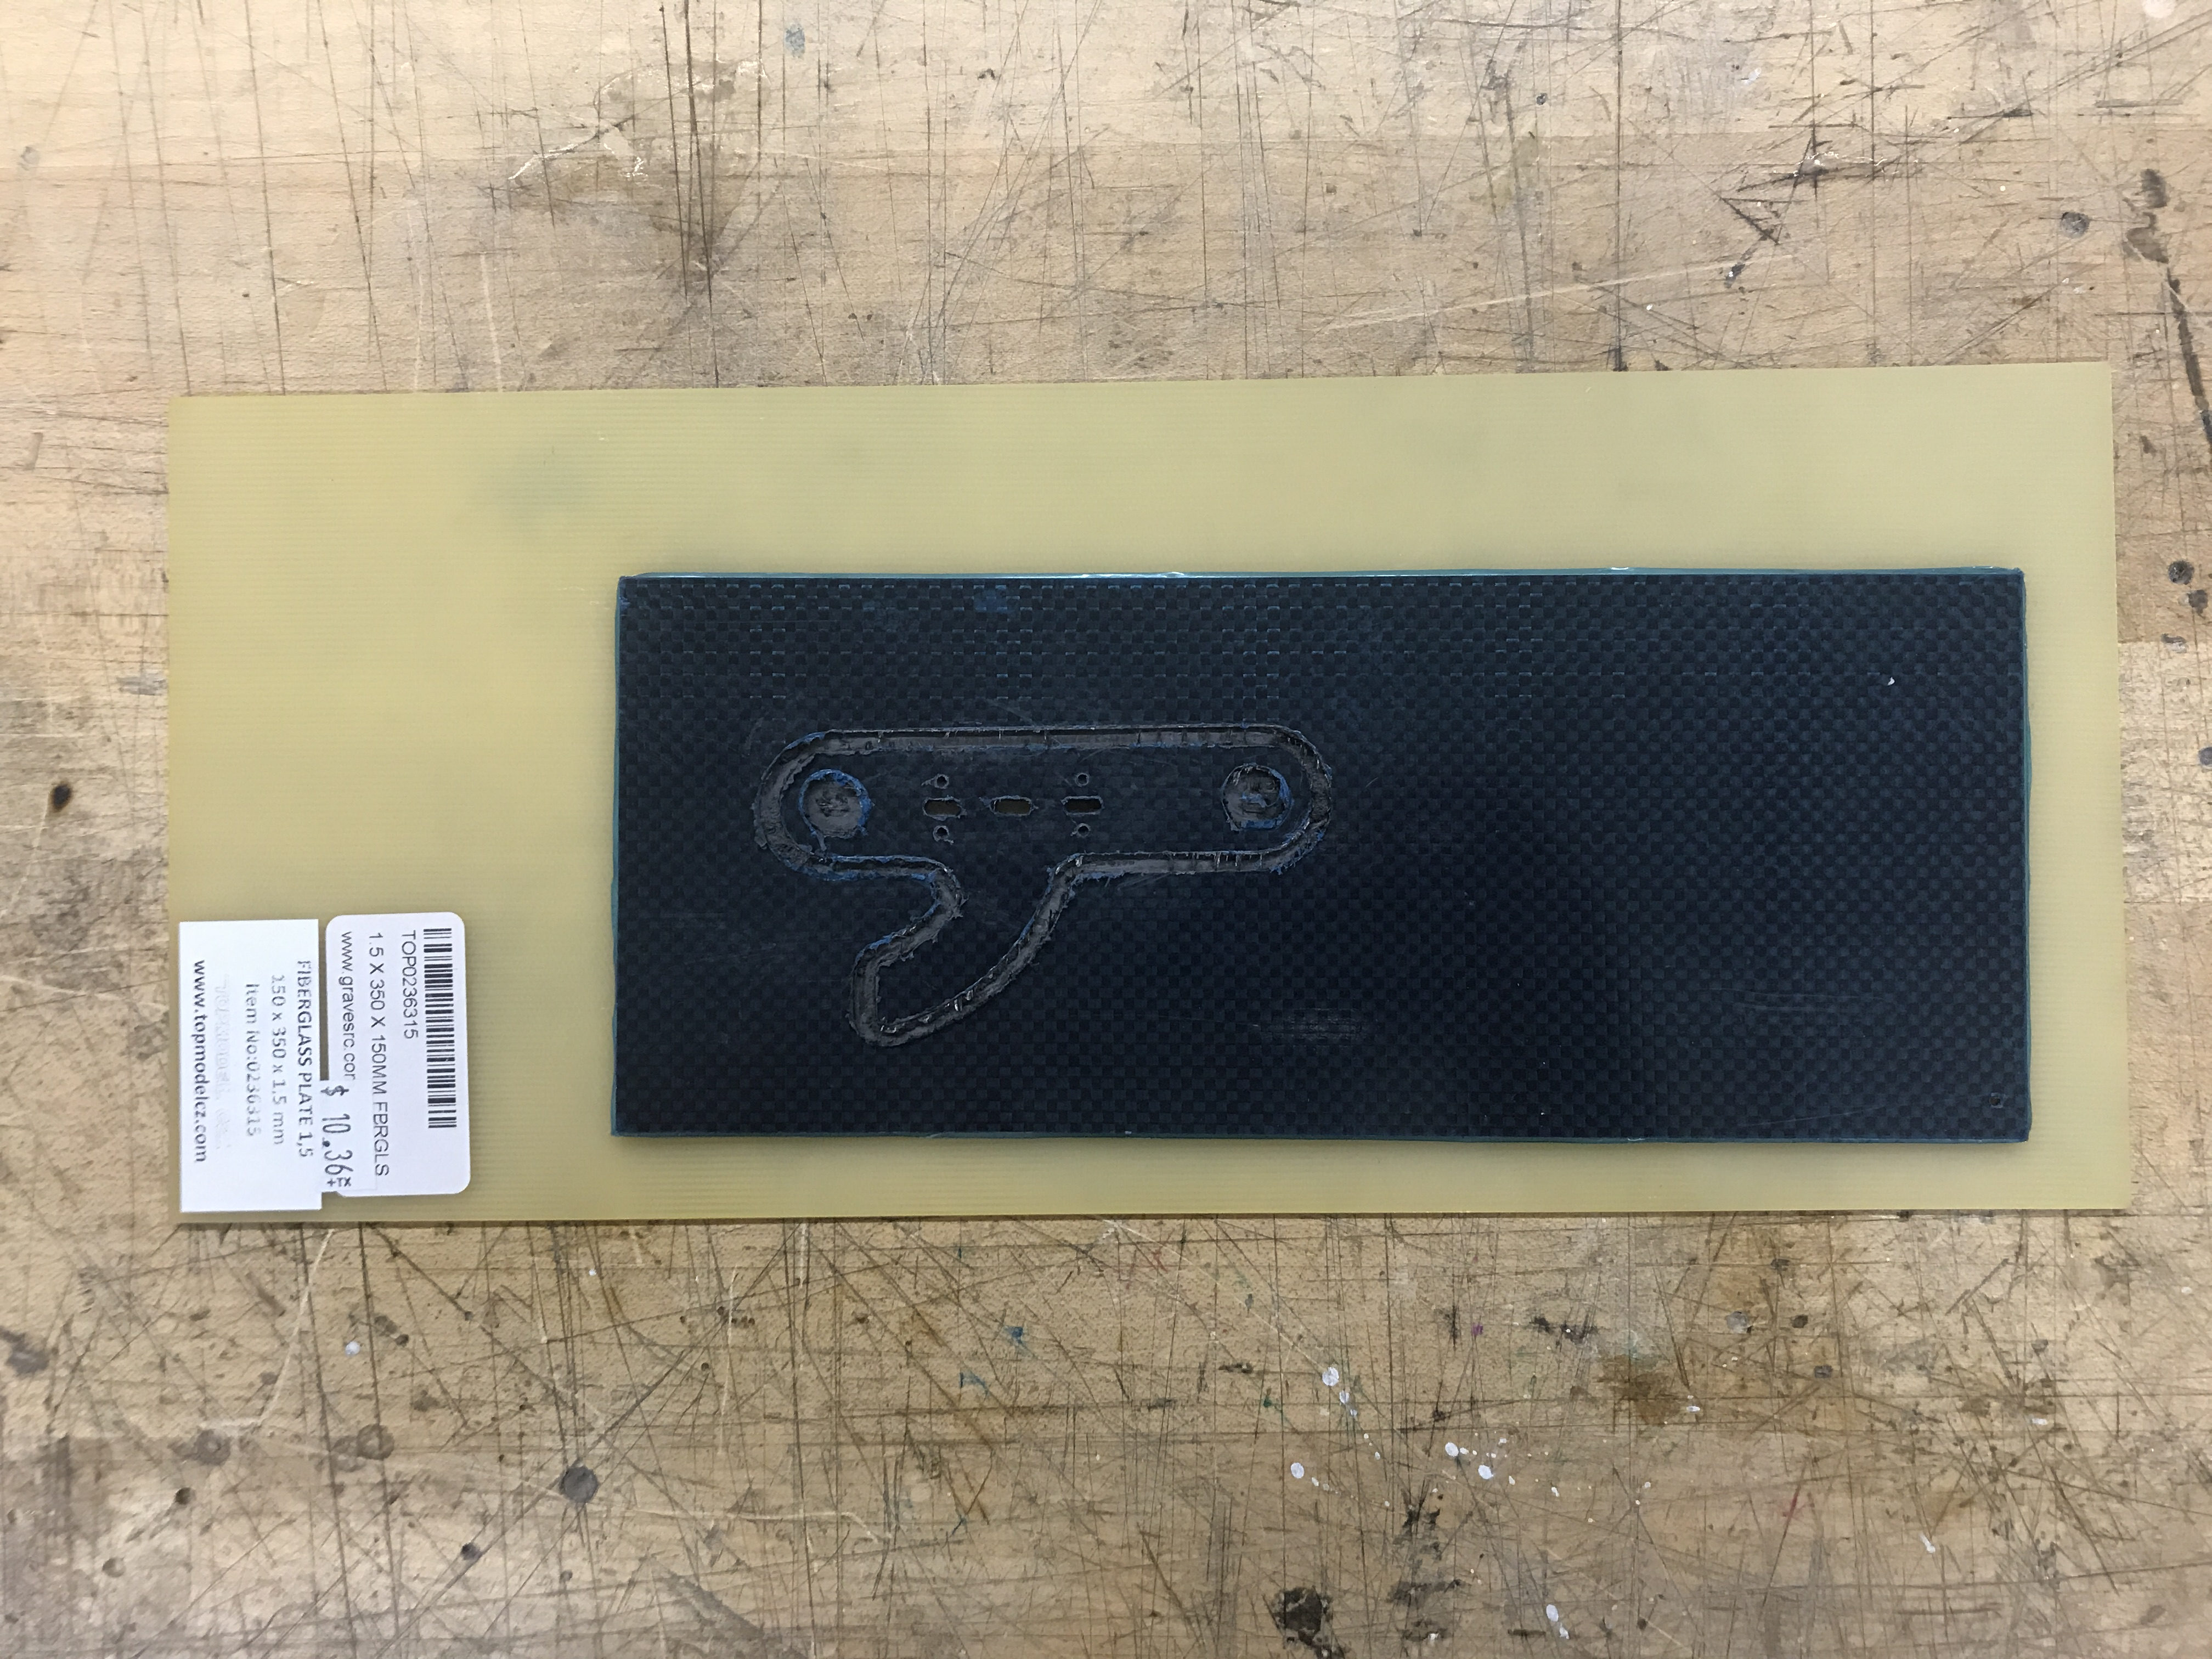
\includegraphics[width=0.95\textwidth, angle=0]{Meetings/March/03-14-22/03-14-22 1.JPG}
\caption{The final cut out of the carbon fiber plate. The drill bit didn't go all the way through.}
\label{fig:031022_1}
\end{figure}

\begin{figure}[htp]
\centering
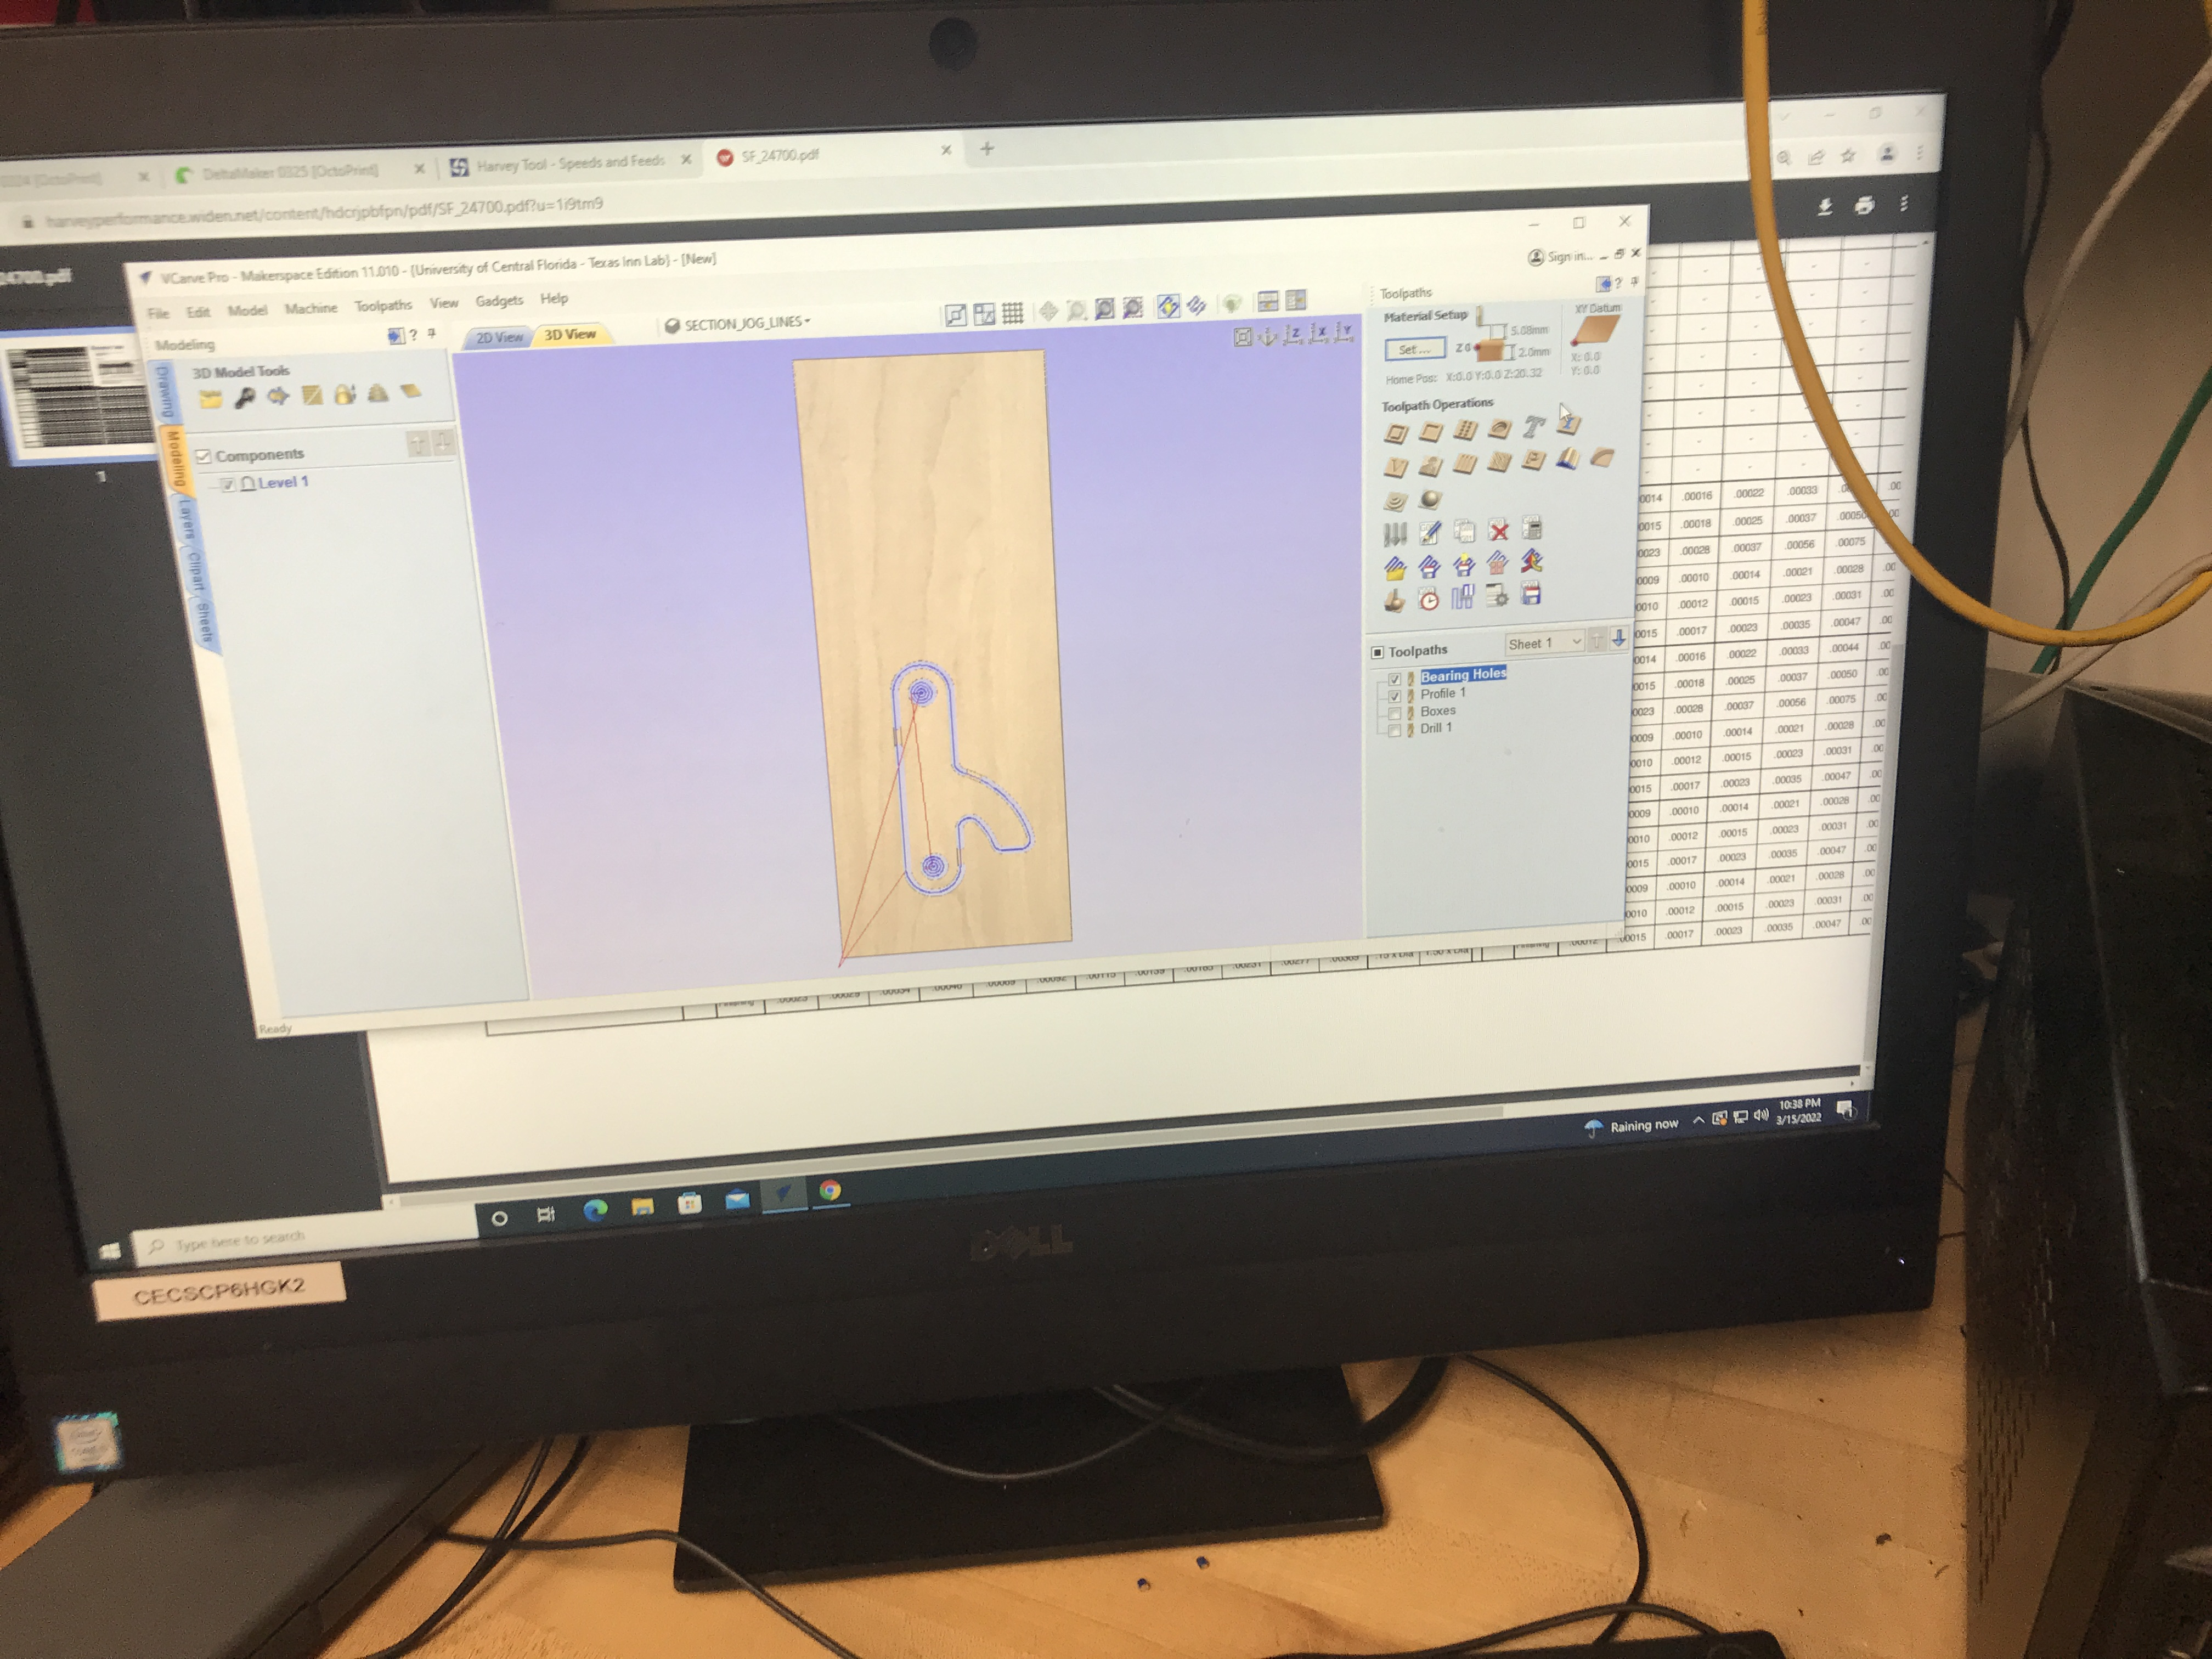
\includegraphics[width=0.95\textwidth, angle=0]{Meetings/March/03-14-22/03-14-22 2.JPG}
\caption{The software we used to prepare the file.}
\label{fig:031022_2}
\end{figure}

\begin{figure}[htp]
\centering
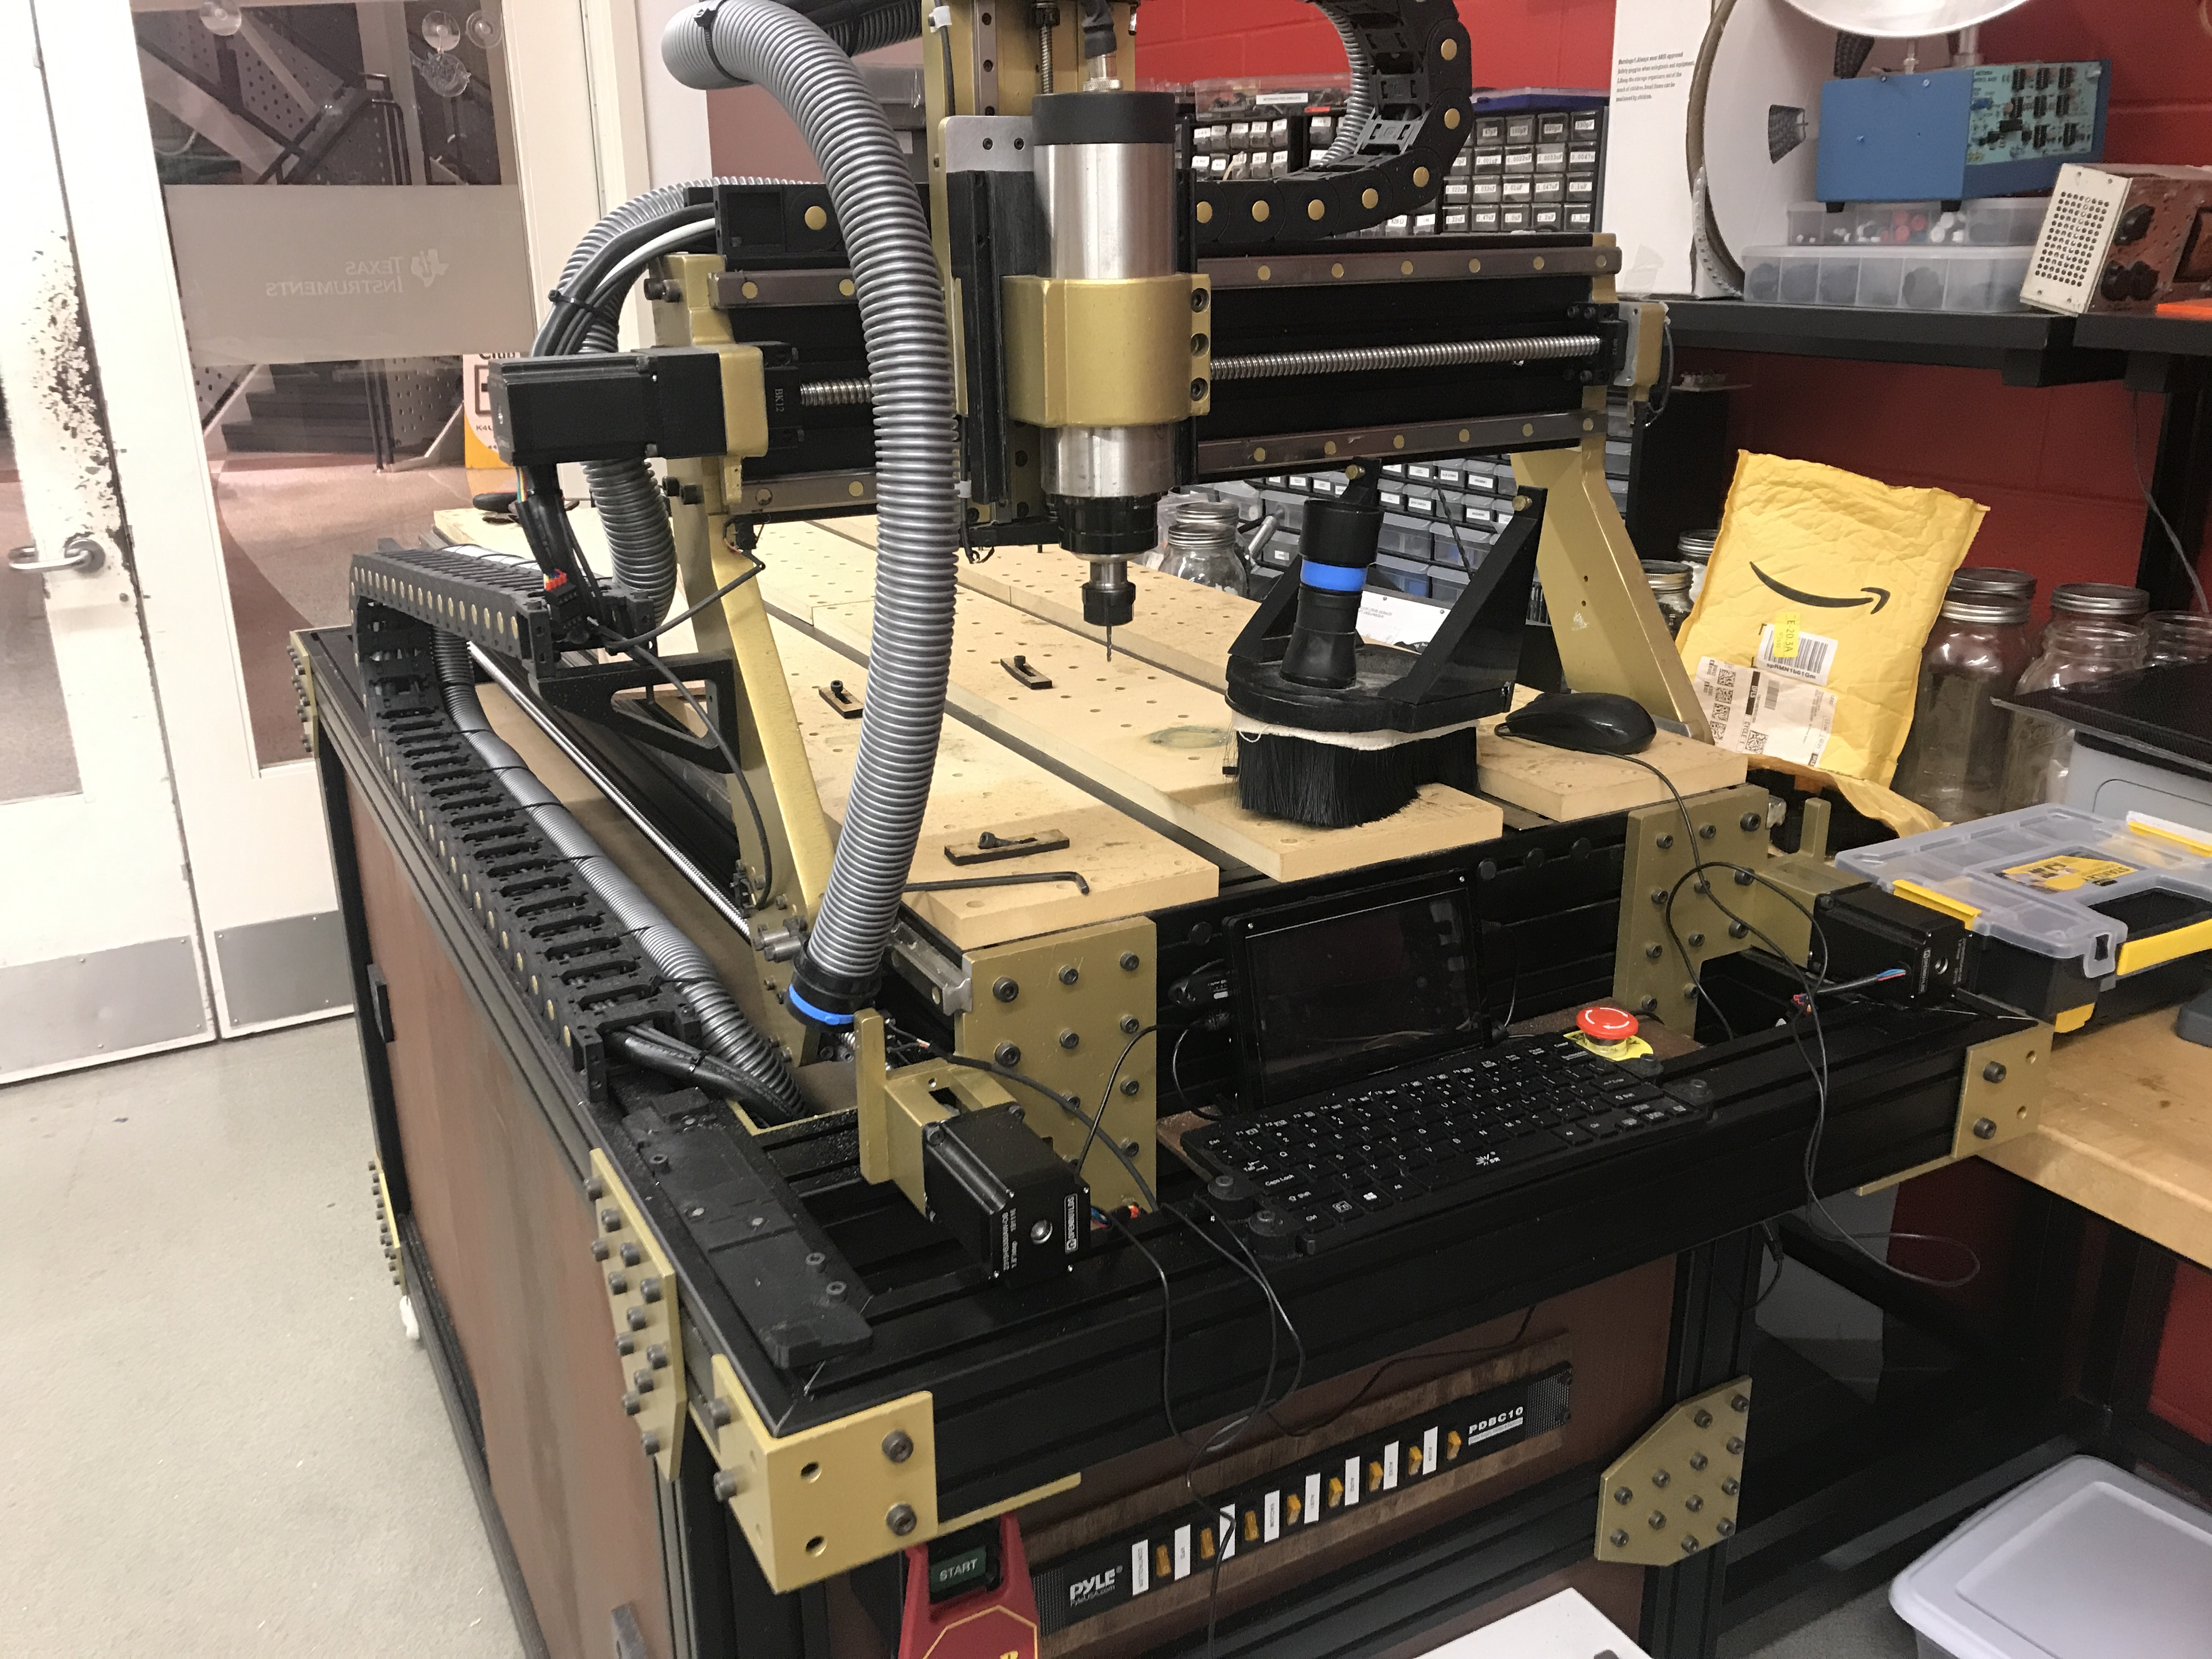
\includegraphics[width=0.95\textwidth, angle=0]{Meetings/March/03-14-22/03-14-22 3.JPG}
\caption{The CNC machine we used.}
\label{fig:031022_3}
\end{figure}

\begin{figure}[htp]
\centering
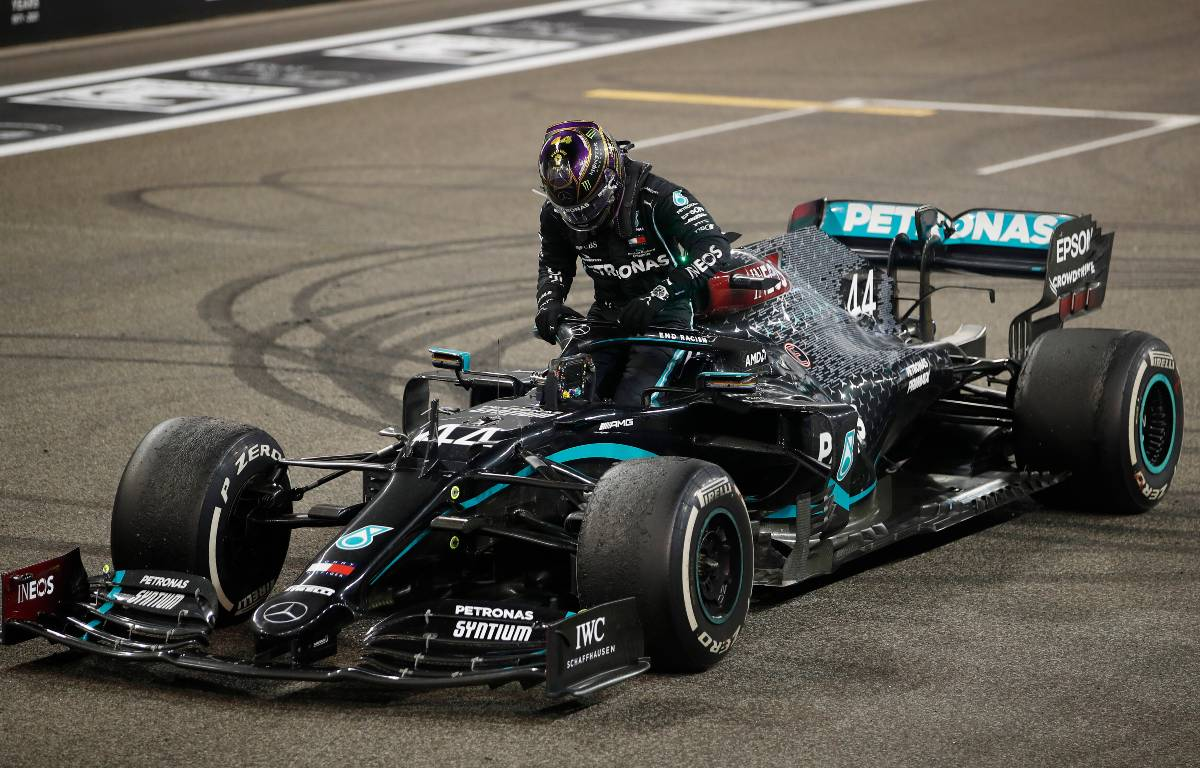
\includegraphics[width=0.95\textwidth, angle=0]{Meetings/March/03-14-22/03-14-22 4.jpg}
\caption{Lewis Hamilton's car also uses carbon fiber.}
\label{fig:031022_4}
\end{figure}






\whatsnext{
\begin{itemize}
    \item Work to improve the autonomous program. 
\end{itemize} 
}

